\documentclass[12pt]{report}

\usepackage[a4paper]{geometry}
%\geometry{left=2.5cm,right=2.5cm,top=2.5cm,bottom=2.5cm, a4paper}
\usepackage[utf8]{inputenc}
\usepackage{amsmath}
\usepackage{amsthm}
\usepackage{amssymb}
\usepackage{ulem}
\usepackage{graphicx}
\usepackage{caption}
\graphicspath{}
\usepackage[document]{ragged2e}
\usepackage{setspace}
\usepackage{tabularx}
\usepackage[slovene]{babel}
\usepackage{textcomp, gensymb}
\usepackage{siunitx}
\usepackage{pdfrender,xcolor}
\usepackage{hyperref}
\usepackage{xurl}
\usepackage{float}
\usepackage{titlesec}

\newfloat{slika}{htbp}{loc}
\floatname{slika}{Slika}

\newfloat{tabela}{htbp}{loc}
\floatname{tabela}{Tabela}

% Differential
\newcommand{\diff}{\mathrm{d}}

\title{
  
\includegraphics[width=0.4\textwidth]{fmf_logo}\\
  {\small Oddelek za fiziko} \\
  {Elektrooptični pojav}\\
  {\small Poročilo pri fizikalnem praktikumu IV}\\

}
\date{}
\author{ Kristofer Č. Povšič \\[5 cm]
 \small Asistentka: Jelena Vesić\\
}


\titleformat{\chapter}[hang]{\Huge\bfseries}{\thechapter{. }}{0pt}{\Huge\bfseries}

\setlength\parindent{0pt}

\begin{document}

\setcounter{page}{2}

\maketitle

\chapter*{Uvod}

Elektrooptični pojav nastane pri vplivu statičnih zunanjih električnih poljih. Obstaja 2 elektrooptična pojava: linearnega, ki se pojavi v anizotropnih snoveh in kvadratnega, ki se pojavi v vseh snoveh. 

V našem primeru imamo homogeno keramiko, pri kateri je mogoč samo kvadratni elektrooptični pojav. Izotropnost keramike je zlomljena z zunanjim električnim poljem. Sprememba lomnega količnika se zgodi na vzporedno z zunanjim poljem polarizirani svetlobi in na svetlobi, ki je polarizirana pravokotno na zunanje polje. 

Ko v keramiko posvetimo s svetlobo valovne dolžine $\lambda$ in spreminjamo zunanje električno polje, se spreminjata v lomna količnika v odvisnosti od kvadrata jakosti električnega polja $E$. Nas zanima samo razlika lomnih količnikov, zato zapišemo: 

\begin{equation}
  n_{\|} - n_{\perp} = B \lambda E^2
\end{equation}

kjer je konstanta $B$ Kerrova konstanta. 

Linearni polarizatorji svetlobo razdeli na dve lastni valovnji, od katerih bo eno prepuščeno, drugo pa zadušeno. 

V Kerrovi celici imamo elektrooptični material postavljen med dve elektrodi, ki spremenita lomna količnika materiala, ko ju priključimo na napetost in dobimo električno polje jakosti $E = \frac{U}{d}$, kjer je $d$ razdalja med elektrodama. 

Električno polje $\vec{E}$ in smer polarizacije sta oba pravokotna na snop polarizirane svetlobe, ki vpada na celico, in kot med njima znaša $45\degree$. Skozi material se zaradi dveh različnih lomnih količnikov širita dve valova z različnima valovnima številoma $k_{\|}=n_{\|}k_0$ in $k_{\perp} = n_{\perp}k_0$, kjer je $k_0$ valovno število in njegova vrednost znaša $k_0 = \frac{2\pi}{\lambda}$. 

Svetloba z amplitudo električnega polja $\vec{\varepsilon_0}$ se razdeli na dva pravokotna dela $\varepsilon_{\|}$ in $\varepsilon_{\perp}$, ki skozi material potujeta z različnima hitrostma. Žarka iz materiala izstopita z različnima fazama in ju analiziramo s pomočjo polarizatorja, ki jakost svetlobe projicira v izbrani smeri. 

Tok na fotodiodi, ki zazna projeciran žarek polarizatorja znaša 

\begin{equation}\label{eq:ftd}
  I = I_1 \sin^2\left(\frac{\pi B L U^2}{d^2} + \frac{\delta}{2}\right)
\end{equation}

\chapter*{Naloga}

\begin{itemize}
  \item Izmerite kotno odvisnost prepustnosti polarizatorja za linearno polarizirano svetlobo.
  \item Izmerite prepustnost dveh pravokotno postavljenih polarizatorjev, ko mednju postavite še tretji polarizator in ga vrtite. 
  \item Določite Kerrovo konstanto \verb+PLZT+ keramike. 
\end{itemize}

\begingroup
\let\clearpage\relax

\chapter*{Potrebščine}
\begin{itemize}
\item He-Ne plinski laser, $\lambda = 632.8\si{nm}$, linearno polariziran v vertikalni smeri 
\item svetlobni modulator s \verb+PLZT+ keramiko, izvor visoke napetosti $0-1000\si{V}$, voltmeter (multimeter)
\item fotodioda vezana na namizni multimeter 
\item polarizatorji (polaroidni filtri) pritrjeni na vrtljivih nosilcih
\item prenosnik št. 5 s programom \verb+ElOpt+, napisanim v LabView-u.
\end{itemize}

\chapter*{Navodilo}

Prižgem He-Ne laser, da se segreje in stabilizira. Potrebščine postavim kot je podano v navodilih. 

\begin{enumerate}
  \item Pred laser postavim en polarizator, poiščem lego, kjer je prepustnost minimalna in maksimalna. Njuna razlika je $90\degree$. V korakih po $5\degree$ vrtim polarizator in si na računalniku beležim vrednost toka na multimetru v odvisnosti od kota zasuka. Skozi točke narišem krivuljo 
  \begin{equation}
    P_p = P_1 \sin^2(\alpha + \delta) + P_0
  \end{equation}

  kjer so $P_1$, $P_0$ in $\delta$ prilagoditvene konstante. 
  \item Prvi polarizator nastavim tako, da je prepustnost minimalna. Za njega postavim drug polarizator in se ponovno po korakih za $5\degree$ sprehodim čez celoten obseg merilnika kota in si beležim vrednosti toka na multimetru. Skozi točke narišem krivuljo 
  \begin{equation}
    P_p = P_1\sin^2(2\beta + \delta) + P_0
  \end{equation}
  \item Postavim Kerrovo celico, da laserski snop sije skoznjo. Vklopim visokonapetostni izvor in multimeter. Izmerim odvisnost prepuščene moči od napetosti v celotnem obsegu visokonapetostnega izvora. Dobljen graf bi moral biti regresija enačbe \ref{eq:ftd}
\end{enumerate}

\endgroup

\chapter*{Obdelava podatkov}

\section*{Polarizator/polarizatorja}

\begin{slika}[H]
  \centering
  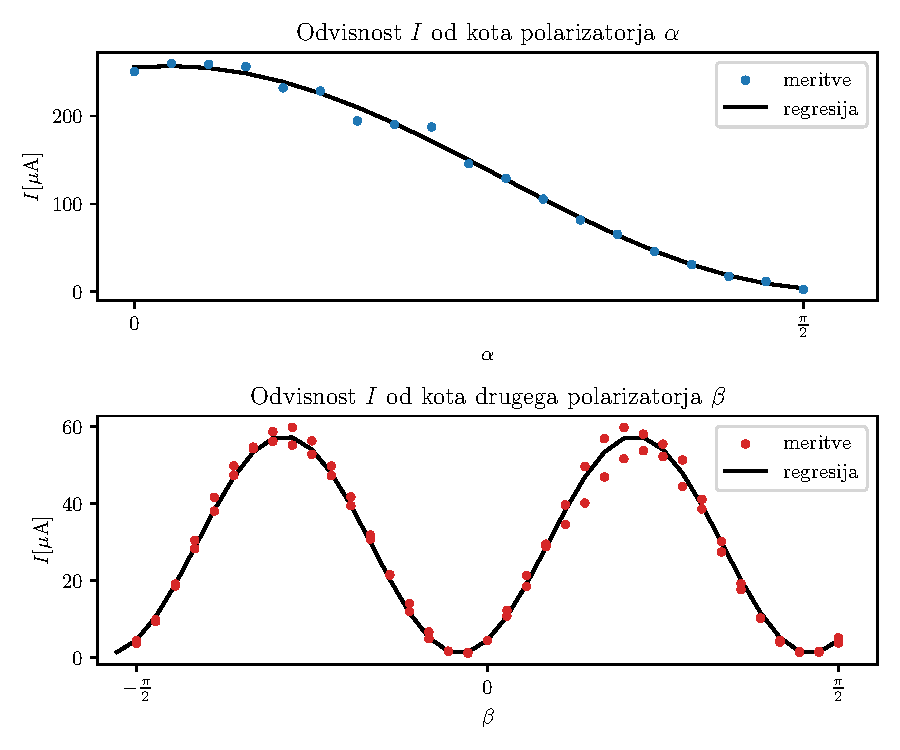
\includegraphics{angleofthedangle}
  \caption{\small Grafa prikazujeta odvisnost toka $I$ od kota polarizatorja in njuni regresiji.}
\end{slika}

Parametri za prvi graf so:

\begin{align*}
  I_{1\alpha} &= (-255 \pm 5)\si{\mu A} \\
  I_{0\alpha} &= (257 \pm 3)\si{\mu A}  \\
  \delta_{\alpha} &= (94 \pm 1)\degree
\end{align*}


Omenil bi, da nisem izmeril za celoten obesg prvega polarizatorja, ampak samo za vrednosti od maksimalne pri kotu $\alpha = 0$ do minimalne vrednosti pri kotu $\alpha = 90\degree$. 

Parametri za drugi graf so: 

\begin{align*}
  I_{1\beta} &= (-56 \pm 1)\si{\mu A} \\
  I_{0\beta} &= (57 \pm 1)\si{\mu A}  \\
  \delta_{\beta} &= (75 \pm 1)\degree
\end{align*}


\section*{Kerrova celica}

\begin{slika}[H]
  \centering
  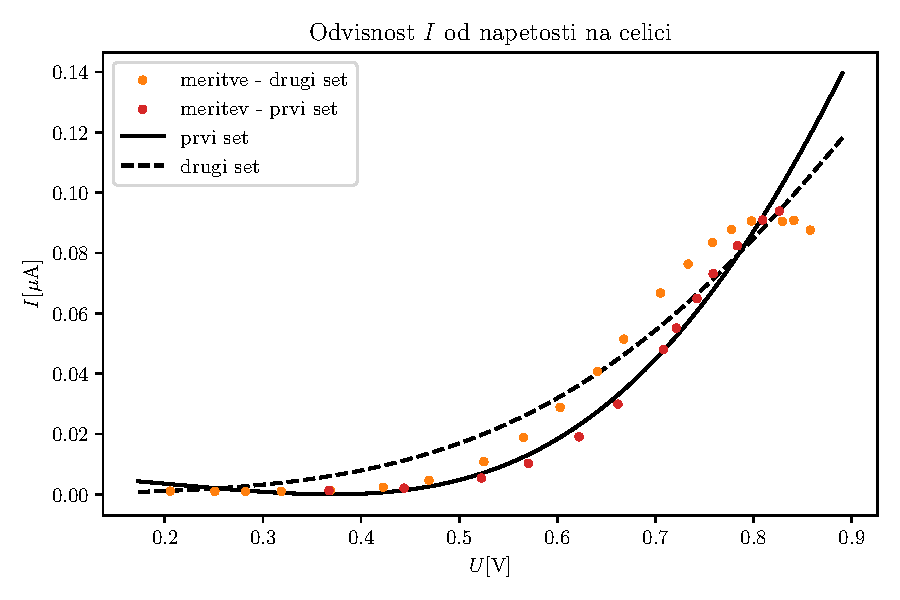
\includegraphics{3naloga}
  \caption{\small Graf prikazuje odvisnost toka $I$ od napetosti $U$ v Kerrovi celici. Regresiral sem dve seriji podatkov: eno ko sem zviševal napetost in drugo, ko sem jo nižal.}
\end{slika}

Parametri za prvi set meritev so: 

\begin{align*}
  I_{1} &= (-37 \pm 1)\si{\mu A}\\
  B &= (0.9 \pm 0.1)\si{\mu A} \\
  \delta_{\beta} &= (23 \pm 1)\degree
\end{align*}


Parametri za drugi set meritev so: 

\begin{align*}
  I_{1} &= (-21 \pm 1)\si{\mu A} \\
  B &= (1.0 \pm 0.1)\si{\mu A}  \\
  \delta_{\beta} &= (-4 \pm 1)\degree
\end{align*}

Prvi set meritev se bolje prilega meritvam kakor drugi, vendar nobeden od njiju se v visokih napetostih ne prilega meritvam (doseg maksimuma in sprememba pregiba funkcije).


\end{document}